\chapter{Detector Calibration System}
\label{chap:DCS}

As described in \autoref{ssec:Particle Detectrion with Bolometers} and shown in \autoref{fig:Sample_pulse}, the actual values that CUORE detects are the changes in resistance of the NTDs as the crystals change temperature due to particles depositing energy.
However, this energy response is strongly non-linear and needs to be calibrated along a range of energies.
Therefore, in order to calibrate these NTD responses to energy depositions in the crystals, and considering the 5 keV energy resolution goal for CUORE, the Detector Calibration System (DCS) was developed.
This system enables the experiment to independently characterize the thermal response over a range of energies up to and beyond the Q-value of \zeronubb~for each of the 988 \teotwo~crystals in CUORE.
This is done by occasionally inserting radioactive sources with known intensity and composition, viz. $^{232}$Th, that emit mono-energetic particles such as photons that will deposit energy into the detectors.
The thermal response of the detectors can then be mapped one-to-one with these known energies, and thus the entire detector array can then be individually calibrated. The hardware and simulation for this work in described in this chapter, and a discussion of how the software analyzes calibrations is described in \autoref{ssec:Calibration}.

\section{Overview}

Making such a system as the DCS, that can meet this goal in the CUORE cryostat is an enormous technical challenge.
As noted in \autoref{sec:Predecessor Experiments} and shown in \autoref{fig:CUORE-0_cryostat_schematic}, calibration sources in CUORE-0 and Cuoricino could be deployed by hand inside the innermost lead shielding to irradiate a single tower of detectors.
However, with 19 towers of crystals making up the CUORE detector array, and with thicker layers of shielding, efficiently deploying sources inside the cryostat requires the sources to be placed in between the towers and inside the roman lead shielding.
This significantly adds to the challenge of such a system as the calibration sources need to be both inserted and retracted from the coldest region of the cryostat on a regular basis.
The main challenges can be summarized as follows: 
\begin{itemize}
\item Calibrate all 988 crystals in as short a time as possible
\item Minimize thermal disturbance to the crystat and the crystals
\item Negligibly contribute to the background in operation
\end{itemize}

The solution to these issues was the Detector Calibration System developed at Wisconsin and at Yale.
With this system, shown in \autoref{fig:DCSintegration}, 12 Kevlar strings containing copper capsules with 2\% thoriated tungsten wire are inserted into the cryostat from above the 300-K stage down into the detector region at the 10-mK and 50-mK stages. 

\begin{figure}[htbp]
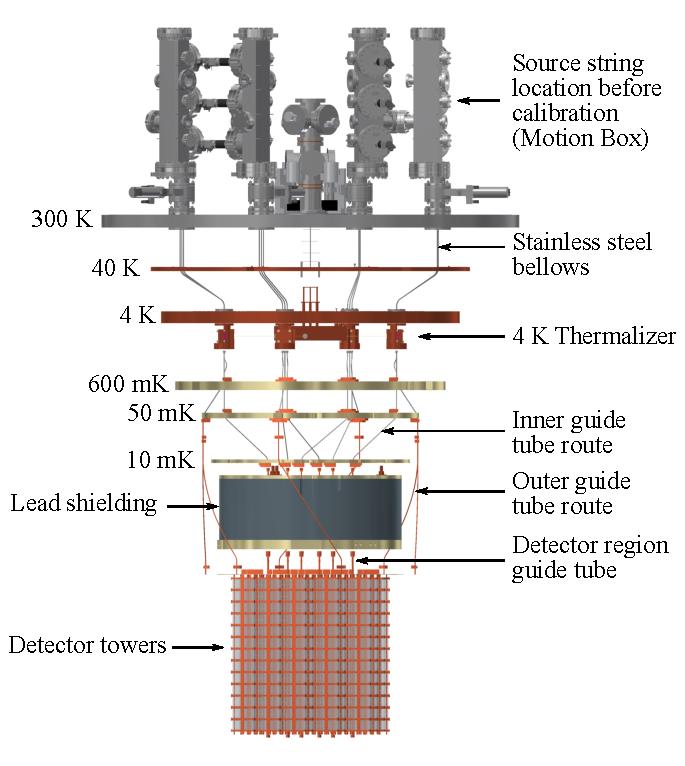
\includegraphics[width=\linewidth]{Figures/DCSintegration.pdf}
\caption[The CUORE Detector Calibration System (DCS).]
{The CUORE Detector Calibration System (DCS).
12 kevlar strings are deployed intermittently into the cryostat through individual tubes through the stages of the cryostat.
6 of the strings are deployed through the inner guide tubes into the 10 mK region of the cryostat between the detector towers, and the other 6 strings are deployed outside the towers in the 50 mK region.
Figure from \cite{Cushman:2016cnv}.}
\label{fig:DCSintegration}
\end{figure}

\section{Calibration Hardware}

The DCS can be divided into a few separate hardware components: the 12 source strings, the 12 sets of guide tubes for the string in the cryostat, the 4 motion boxes, the 4-K thermalization system, and the cabling for the software control system.
Each of these sets of components has different technical challenges, particularly for the calibration tubes nearest to the detectors that have stringent radioactivity requirements, and are described in more detail in this section.

\subsection*{Calibration Source Strings}
There are 12 calibration source strings that are deployed in to the detector region in order to calibrate the 19 towers of CUORE.
These source strings consist of copper capsules covered in PTFE heat shrink tubing that enclose the 2\% thoriated tungsten source inside, shown in \autoref{fig:source_carrierA}.
The copper is crimped on top and bottom in order to hold it onto the Kevlar string and to hold the source inside, and the Teflon heat shrink reduces the friction between the copper capsules and the DCS guide tubes. In addition, the bottom 8 capsules have reducing spacing and are wider than the other capsules, shown in \autoref{fig:source_carrierB}.
As the sources are deployed into the cryostat under their own weight, these heavier capsules (called ``weight" capsules, opposed to the other ``source" capsules\footnote{Despite the naming convention, all the copper capsules contain radioactive sources.}), and particularly the PTFE guide ball, assist the strings with lowering into the funnels between stages and in detecting obstructed paths.
For example, if the tubes are not perfectly vertically centered, the guide ball will be caught by the funnel and guide the string down into the funnel, where the weight of the capsules will pull the string down into the funnel correctly.
This is opposed to a case where, if there were no weight capsules, some string would fall into the tube, but the rest would drape off the side of the funnel and fail to deploy since the string would not be sufficiently pulled down into the tube.

\begin{figure}[htpb]
\begin{center}
\begin{subfigure}[b]{0.60\textwidth}
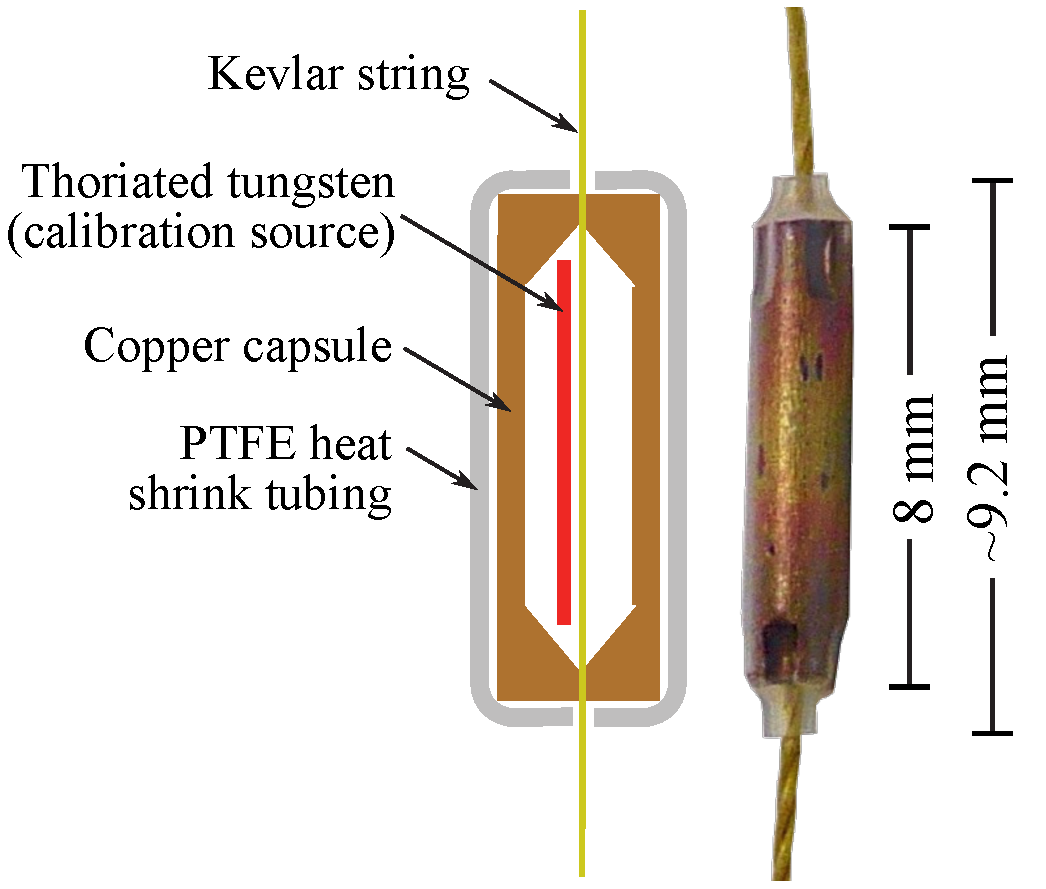
\includegraphics[height=2.2in]{Figures/source_capsule_schematic.pdf}
\caption{}
\label{fig:source_carrierA}
\end{subfigure}
\begin{subfigure}[b]{0.15\textwidth}
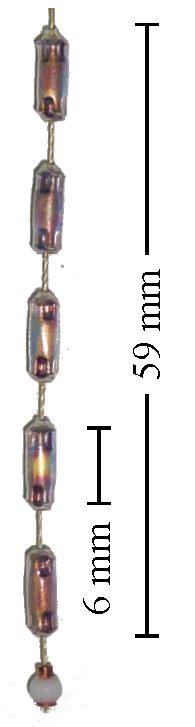
\includegraphics[height=2.7in]{Figures/string_bottom.pdf}
\caption{}
\label{fig:source_carrierB}
\end{subfigure}
\end{center}
\caption[(a) Schematic and photograph of an assembled source capsule. (b) Photograph of five heavier bottom capsules and PTFE ball at the bottom of a source string.]{(a) Schematic and photograph of an assembled source capsule. (b) Photograph of five heavier bottom capsules and PTFE ball at the bottom of a source string.}
\label{fig:source_carrier}
\end{figure}
 
Recalling that one of the design goals for the DCS is to calibrate all 988 crystals in as short a time as possible, the strings are configured, when fully deployed in the cryostat, to optimize coverage on all the crystals, as the time it takes to calibrate the detector array is limited by the time it takes the least-irradiated crystals to calibrate.
To this end, the calibration sources are configured in a double-hexagonal pattern, as shown in \autoref{fig:Calibration_source_top_view} with the inner source strings inside the 10-mK vessel irradiating the towers and floors closest to the center and the outer strings outside the 50-mK vessel irradiating the towers and floors furthest from the center.
The inner calibration strings are located about 2 cm from the faces of the crystals, and the outer calibration strings are about 18 cm away from the crystals, although they are shielded from the crystals by the 10-mK and 50-mK vessel.
As a result of this geometry, there are two main differences between the copper capsules in each calibration string and between the inner and outer strings, viz., the bottom and top capsules of each string have a boosted activity relative to the capsules in the middle of the string, and the capsules in the outer strings have a boosted activity relative to their counterparts in the inner strings, with the specific activities of each described in \autoref{tab:calibration_activities}
In addition, there is one more capsule on the inner strings relative to the outer strings, which is due to the fact that when the strings were made, the activities were lower than anticipated and needed a more significant boost at the top of the calibration string.
The reason for this asymmetry for the activity of the capsules on each string is to have roughly equal rates on each crystal on each floor, and, since the calibration strings are only slightly longer than the towers themselves\footnote{The inner and outer calibration strings have an active region 80 and 83 cm long, respectively.}, these edge effects need to be considered for optimal calibration.
The spacing of the source capsules is designed such that each floor sees roughly 2-3 adjacent capsules at a time, and the vertical geometry of the strings in their nominal vertical positions is shown in \autoref{fig:Calibration_source_tower}.

\begin{figure}[htpb]
\begin{center}
\begin{subfigure}[b]{0.5\textwidth}
    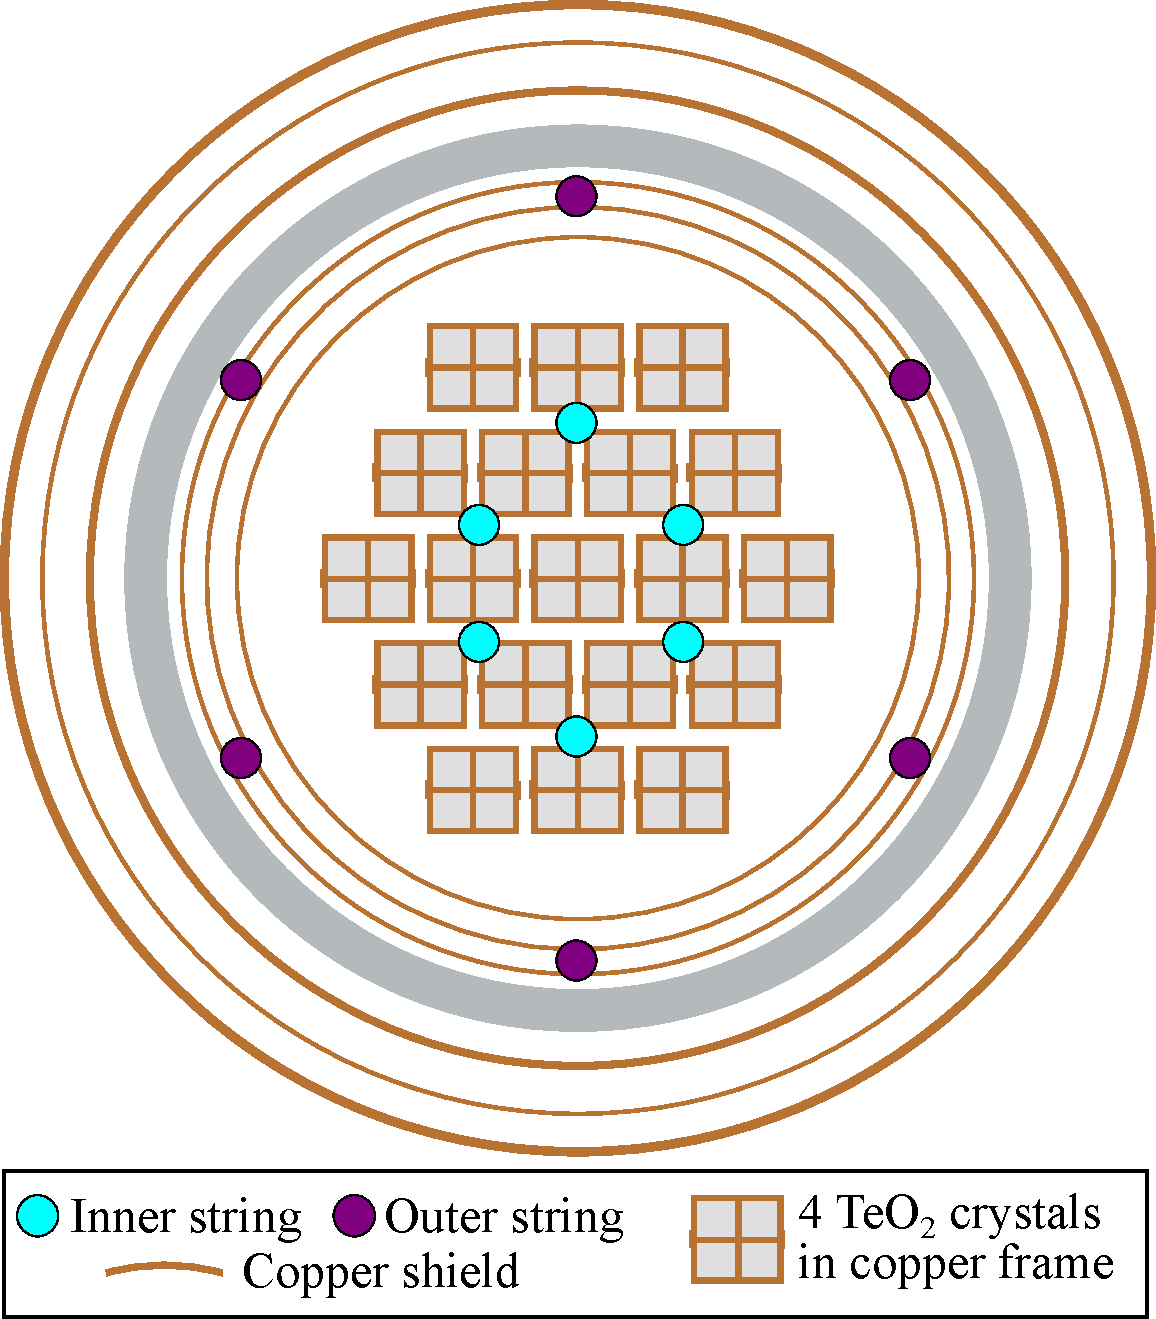
\includegraphics[height=3.25 in]{Figures/CUORE_calibration_location.pdf}
    \caption{}
    \label{fig:Calibration_source_top_view}
\end{subfigure}
\begin{subfigure}[b]{0.40\textwidth}
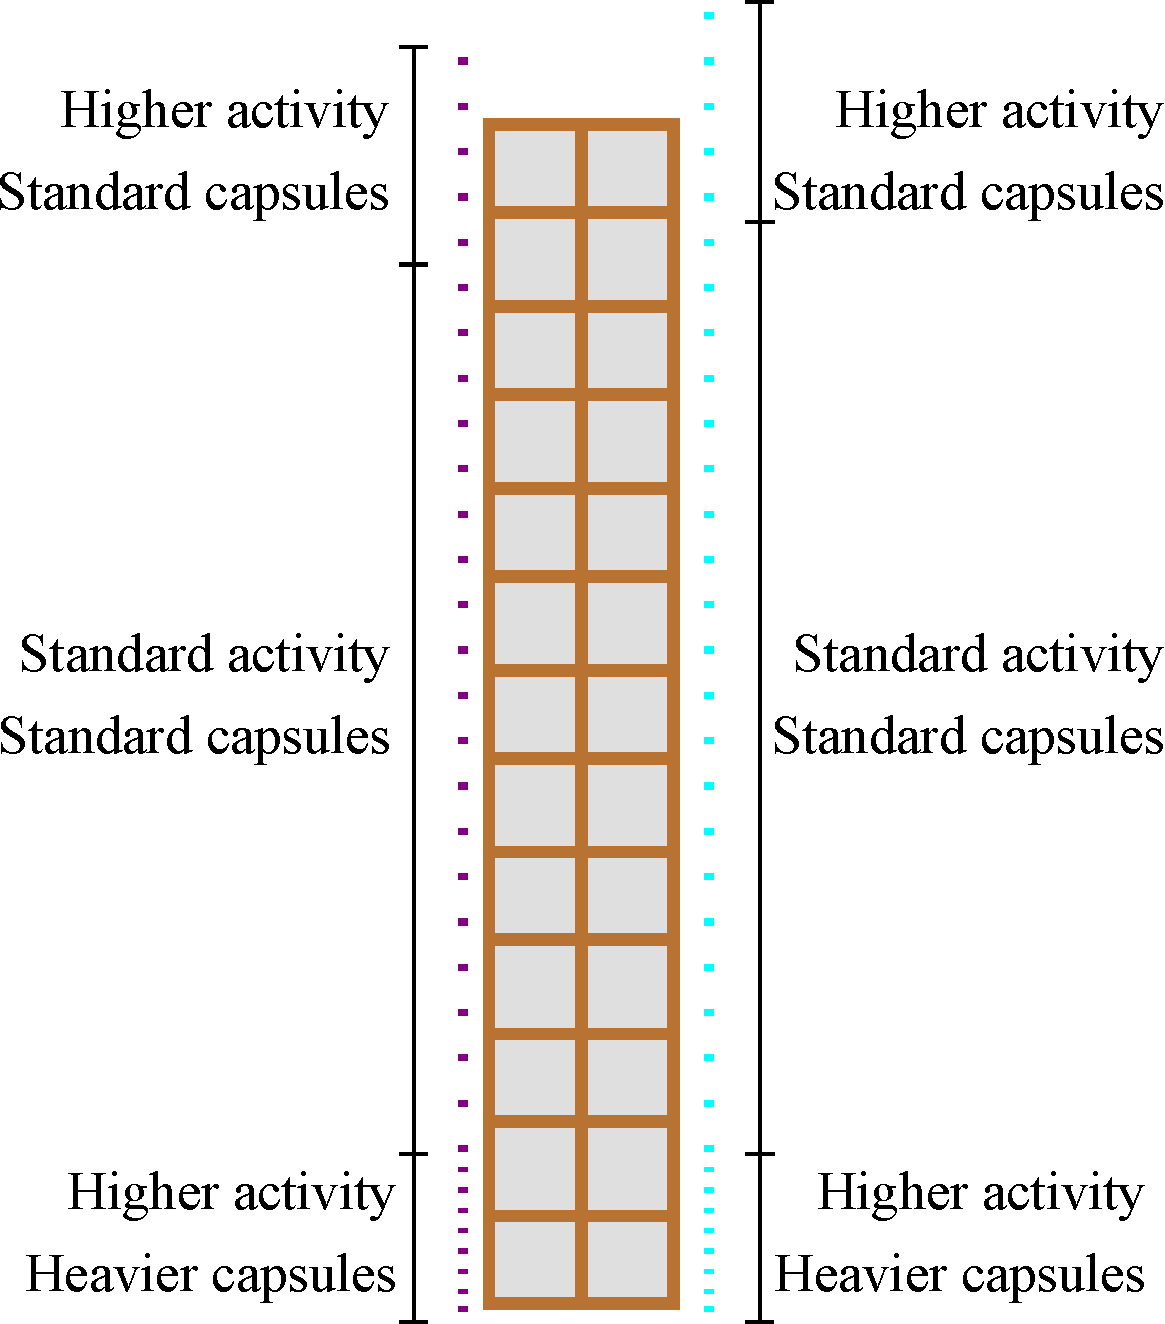
\includegraphics[height = 3.5 in]{Figures/Cuore_tower_calibration.pdf}
\caption{}
\label{fig:Calibration_source_tower}
\end{subfigure}
\end{center}
\caption[(a) A top-down schematic of the calibration source strings in the cryostat.
(b) A side-view schematic of an inner and outer calibration string next to a tower.]
    {(a) A top-down schematic of the calibration source strings in the cryostat.
    The inner strings irradiate the innermost towers, and the outer strings irradiate the outermost towers.
    Due to space constraints, the outer sources are located outside the 50-mK vessel.
    (b) A side-view schematic (horizontal axis not to scale) of a tower with an adjacent inner (right) and outer (left)  calibration string.
    Figures adapted from \cite{Cushman:2016cnv}.}
\label{fig:Calibration_source_locations}
\end{figure}

\begin{table}[htbp]
    \centering
    \caption[The number of capsules and activities of each calibration source.]
    {The number of capsules and activities of each calibration source.
    The capsules are listed from bottom to top, with the 8 capsules corresponding to the weight capsules on the string.
    For the activity, the activity of each capsule is listed, along with the total summed activity of that component.
    In total, the activity of the inner strings is 3.6 Bq, and the activity of the outer strings is 19.4 Bq, with the activities listed as the activity of the $^{208}$Tl decay in the $^{232}$Th decay chain.}
    \label{tab:calibration_activities}
    \begin{tabular}{lccc}
    \hline 
    \hline
        String type & Capsules & Activity (Bq) & Summed Activity (Bq) \\
        \hline 
        \multirow{3}{*}{Outer} & 8 & 0.64 & 5.12 \\
        & 20 & 0.48 & 9.52 \\
        & 5 & 0.95 & 4.75 \\
        \hline
        \multirow{4}{*}{Inner} & 8 & 0.07 & 0.54 \\
        & 21 & 0.09 & 1.95 \\
        & 4 & 0.08 & 0.31 \\
        & 1 & 0.80 & 0.80 \\
        \hline
        \hline
    \end{tabular}
\end{table}

\subsection*{Motion Boxes}
On top of the cryostat, there are four motion boxes, shown in \autoref{fig:motion_box}, that contain the DCS calibration strings while they are not being deployed and the motors that control the motion of the strings.
The motion boxes have dimensions $12.6\times7.9\times60.7~\textrm{cm}^3$ constituting a 6 L volume.
There are three strings in each motion box that are wound up on each of the calibration string spools internally.
These calibration strings can then be deployed independently and simultaneously down through three guide tubes in the motion box down into the cryostat.
Inside the motion boxes, each acts as an independent vacuum system during, only connecting to the IVC when calibration strings are being deployed into the cryostat.
A proximity sensor at the bottom of the motion box detects when the copper capsules enter and disturb the electromagnetic field produced by the sensor.
This allows for us to determine when individual source capsules or the weight capsules\footnote{The sensor is unable to resolve the denser-packed weight capsules and triggers continuously while they are in the sensor.} move either into or out of the motion box.
\begin{figure}[htpb]
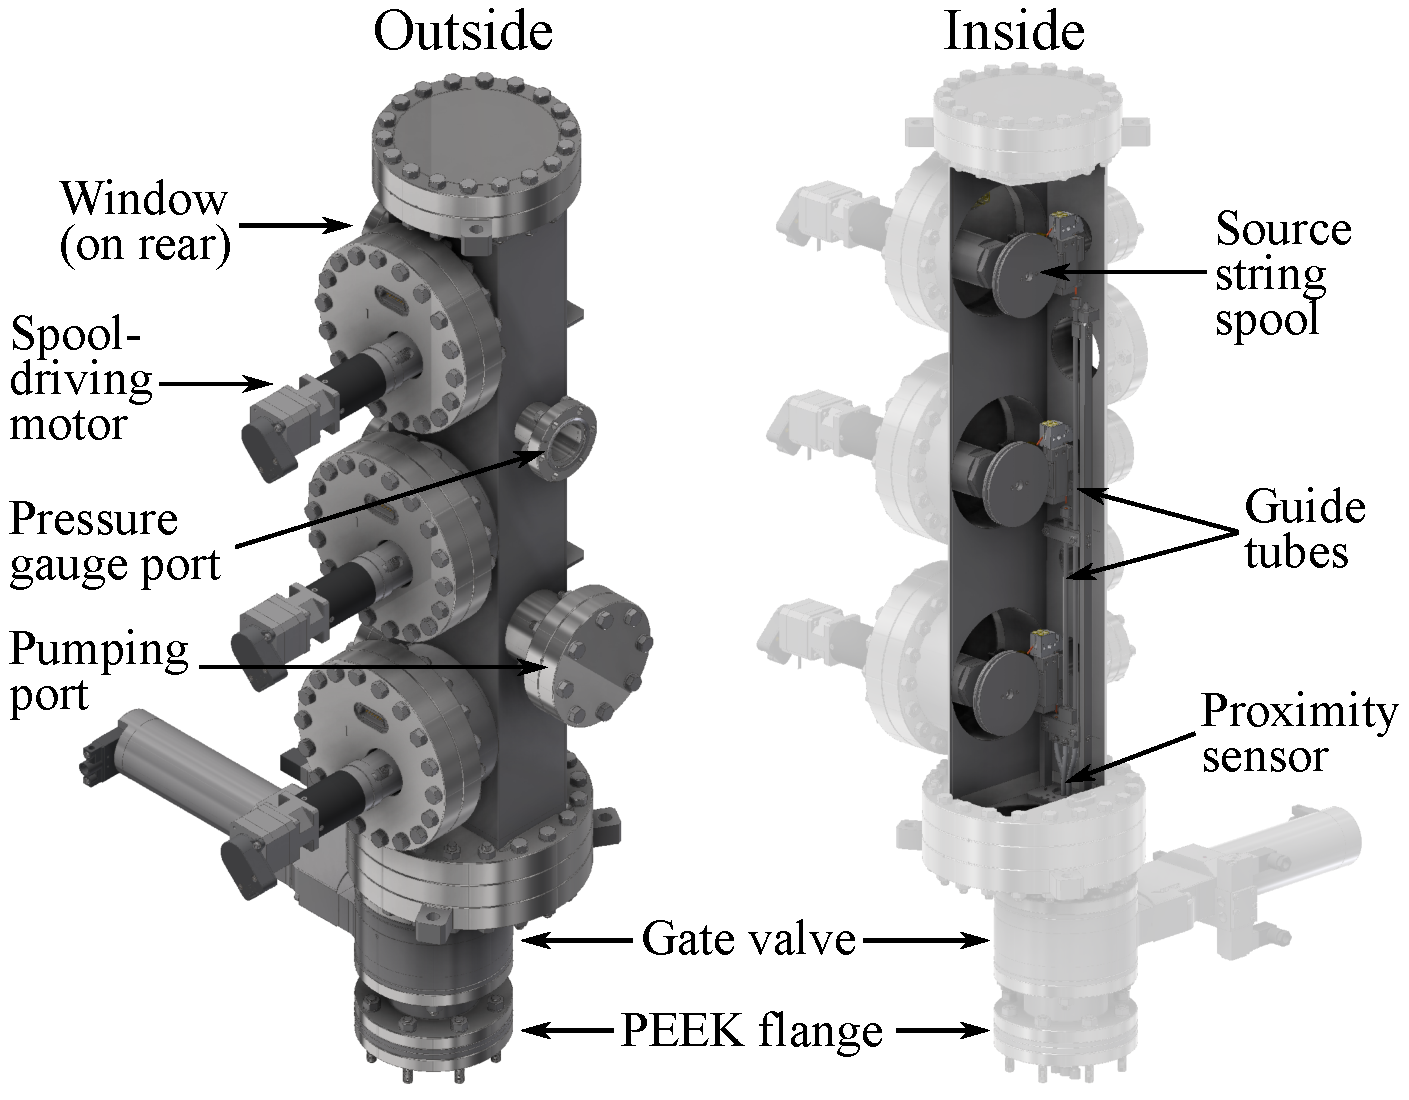
\includegraphics[width=0.9\linewidth]{Figures/motion_box.pdf}
\caption[A rendering of a single motion box from two different angles.]{A rendering of a single motion box from two different angles. The motion box is mounted vertically with the PEEK flange on top of the cryostat with the three source strings spools above. The windows on each motion box allow for the source strings to be observed from outside.}
\label{fig:motion_box}
\end{figure}
The motion box has 3 CF
The motion boxes contain all of the electronic controls that enable and monitor the deployment of the calibration strings into the crystat.

\subsection{Guide Tubes}


\begin{figure}[htbp]
    \centering
    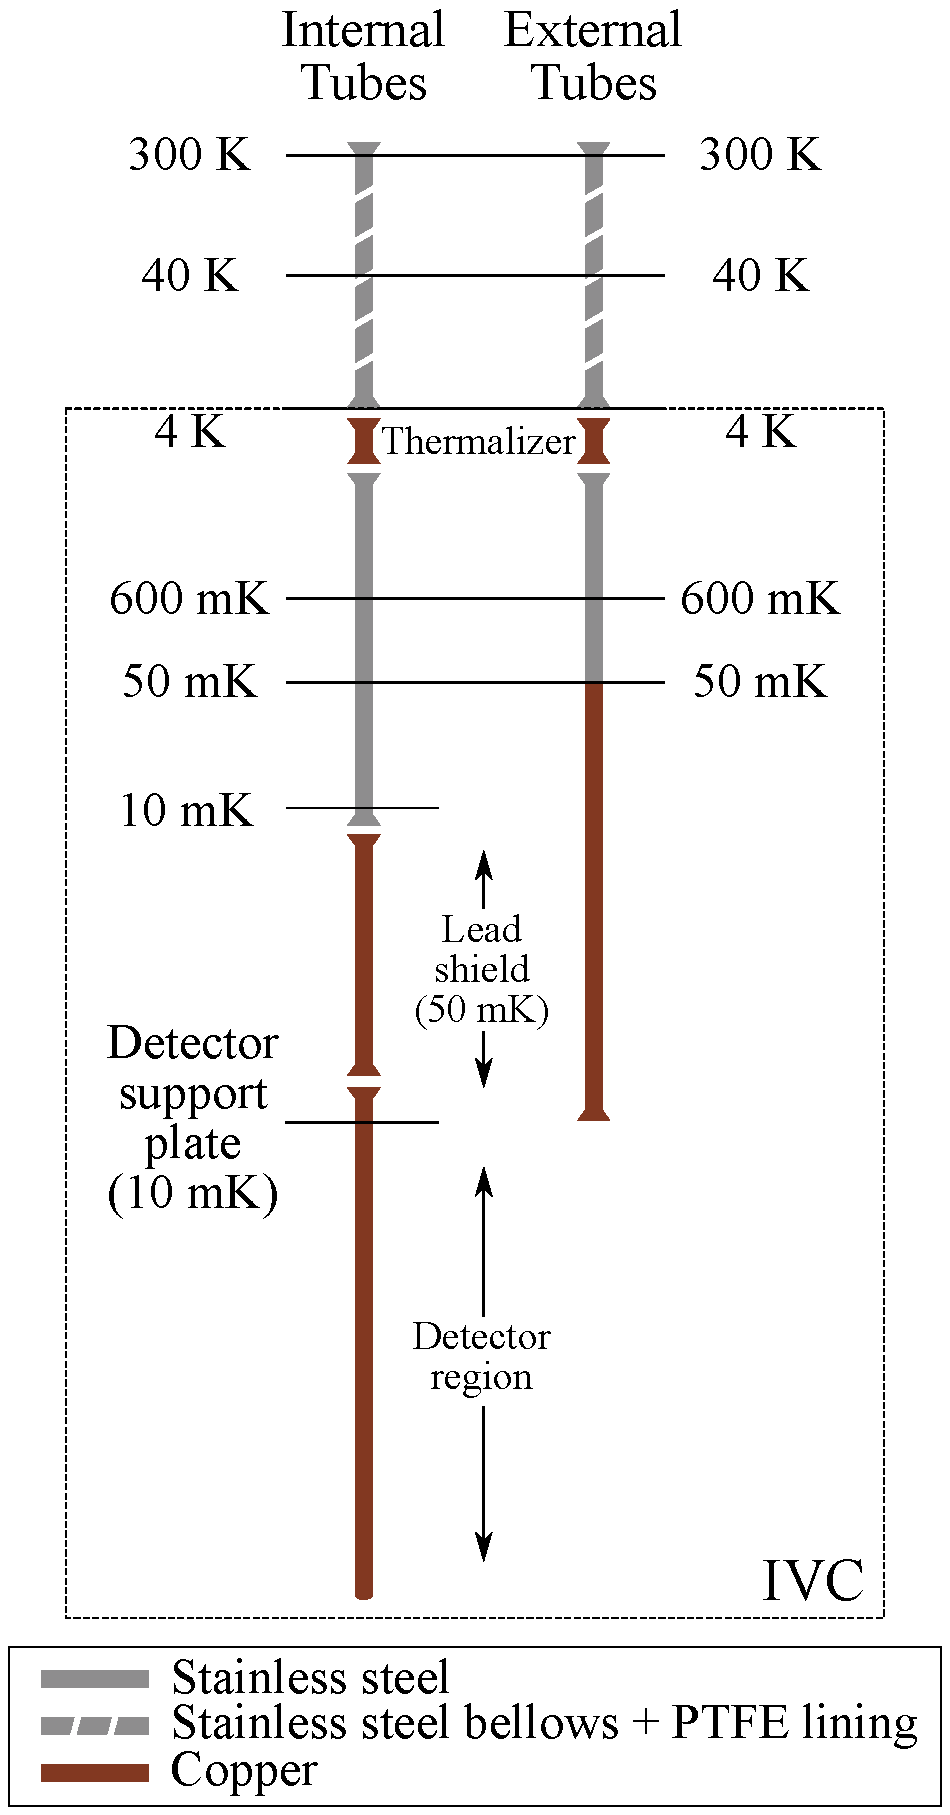
\includegraphics[height=0.4\paperheight]{Figures/thermal_coupling.pdf}
    \caption[A diagram showing the thermal couplings of the DCS tubes for both the internal and external sources.]
    {A diagram showing the thermal couplings of the DCS tubes for both the internal and external sources.
    In order to minimize the thermal load on the cryostat, there are multiple breaks in the DCS tubes with funnels for the calibration sources to pass through.
    Near the detectors, the tubes switch from being stainless steel with low thermal conductivity to low-background copper.
    For the external tubes, there are no tubes below the lead shield and the source capsules hang freely.
    Figure from \cite{Cushman:2016cnv}.}
    \label{fig:dcs_thermal_coupling}
\end{figure}


\subsection{Thermalization and Thermometry}
In order to deploy 12 calibration source strings from 300 K down to 50 or 10 mK, the sources need to be cooled as much as possible before they reach each stage of the cryostat or even the black-body radiation from the sources will cause the temperature of the crystals and the cryostat to rise excessively and possibly dangerously. Most of the mass, and therefore the heat \color{red} find a better word than heat \color{black} is carried in the copper capsules. The kevlar that holds the capsules is a poor conductor of heat \color{red} Citation Needed \color{black} compared with the capsules, which is a necessary feature, in addition to its strength, as the kevlar will form 12 continuous lines from the motion boxes at 300 K down to the detector region at 10 mK.

To effect this cooling on the source strings, multiple methods are used. The main cooling mechanism used is from the copper thermalizers located at the 4 K plate, shown in \autoref{fig:DCS_4K_schematic}. These thermalizers consist of a moving copper block and a copper base, with the copper block pushed away by a spring. The copper block is activated by another kevlar string that, when pulled, pushes the copper block onto the copper base. The cooling time decreases as the force between the copper block and capsule increases, and a force of 32 N was chosen This cooling is performed at the 4K stage as the cryostat has the most cooling power at this stage \color{red} Link to the cooling power table \color{black}. Most of the cooling of the capsules is done at this position and this thermalization process over an entire string is a significant fraction of its total deployment time.


\color{red}connect these figures \color{black}
\begin{figure}[htbp]
    \centering
    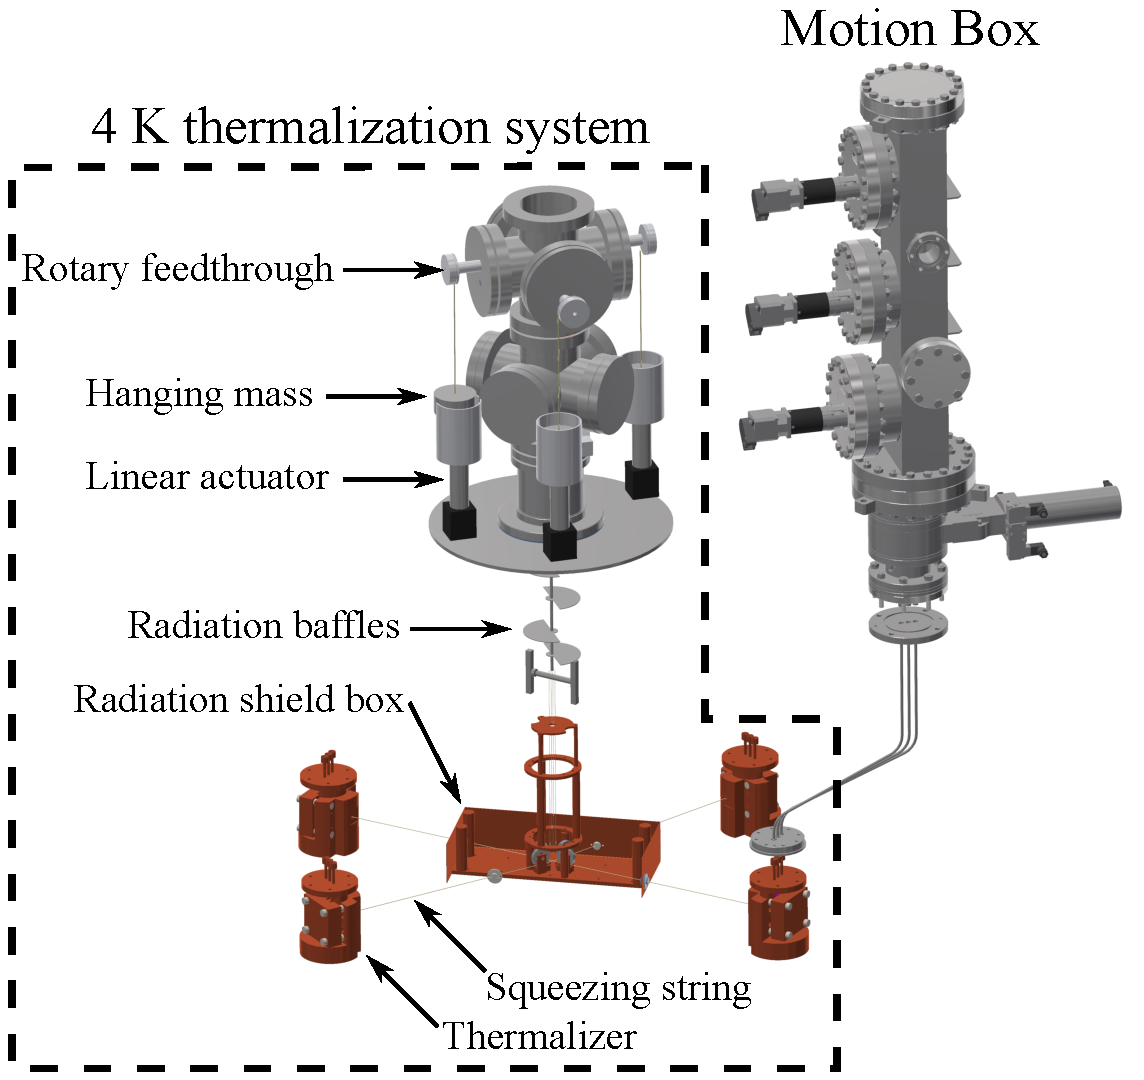
\includegraphics[width=0.8\linewidth]{Figures/thermalization_system_labeled.pdf}
    \caption[A cutaway drawing of the 4-K thermalization system on CUORE.]
    {A cutaway drawing of the 4-K thermalization system on CUORE.
    When the linear actuator is fully down, the hanging mass hangs freely from the rotary feedthrough, which is then connected through a pulley to the copper block.
    This applies the 32 N of force acting on a capsule in order to cool it down to 4 K.}
    \label{fig:DCS_4K_thermalizer}
\end{figure}

\begin{figure}[htbp]
    \centering
    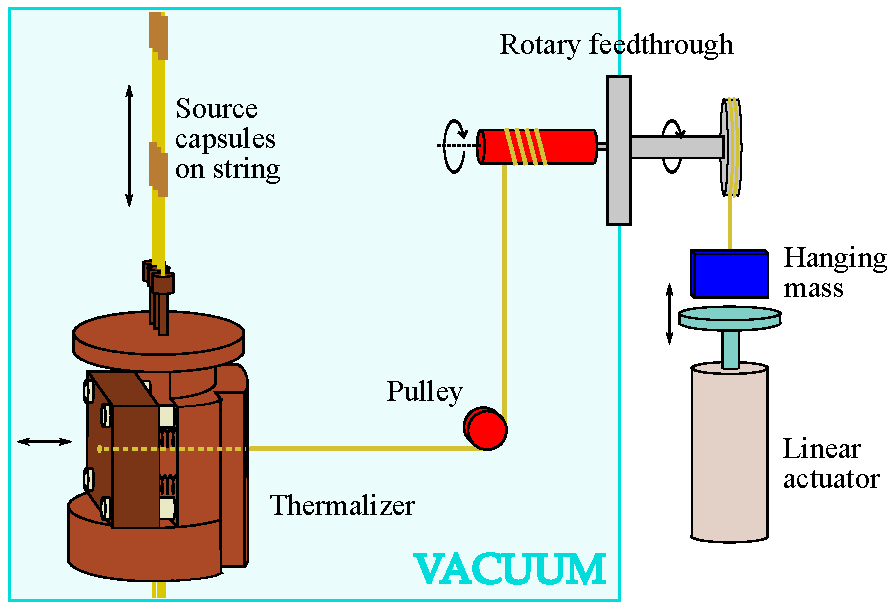
\includegraphics[width=0.8\linewidth]{Figures/Thermalizer_schematic_labeled.pdf}
    \caption{Caption}
    \label{fig:DCS_4K_schematic}
\end{figure}


Another way in that heat is removed from the source strings is due to the contact with the walls of the guide tubes. This cooling, however, is limited in two main ways: by the angle of the tube as steeper angles provide less contact with the source capsule and by the heat capacity and thermal contact of the tube with each stage as some tubes, namely those at 600 mK will warm up to 4K or beyond. Below the thermalizers, the inner strings also go through a ``chicane" \color{red} Should I put this in quotes? Also, add reference to figure\color{black} which increases the contact between the capsules and the tubes. This is done to further increase the rate at which heat is removed from the capsules as the cooling on these sources that are to be deployed at the 10 mK stage are the most critical to cool, but the cooling power decreases at colder stages. 

\begin{figure}[htbp]
    \centering
    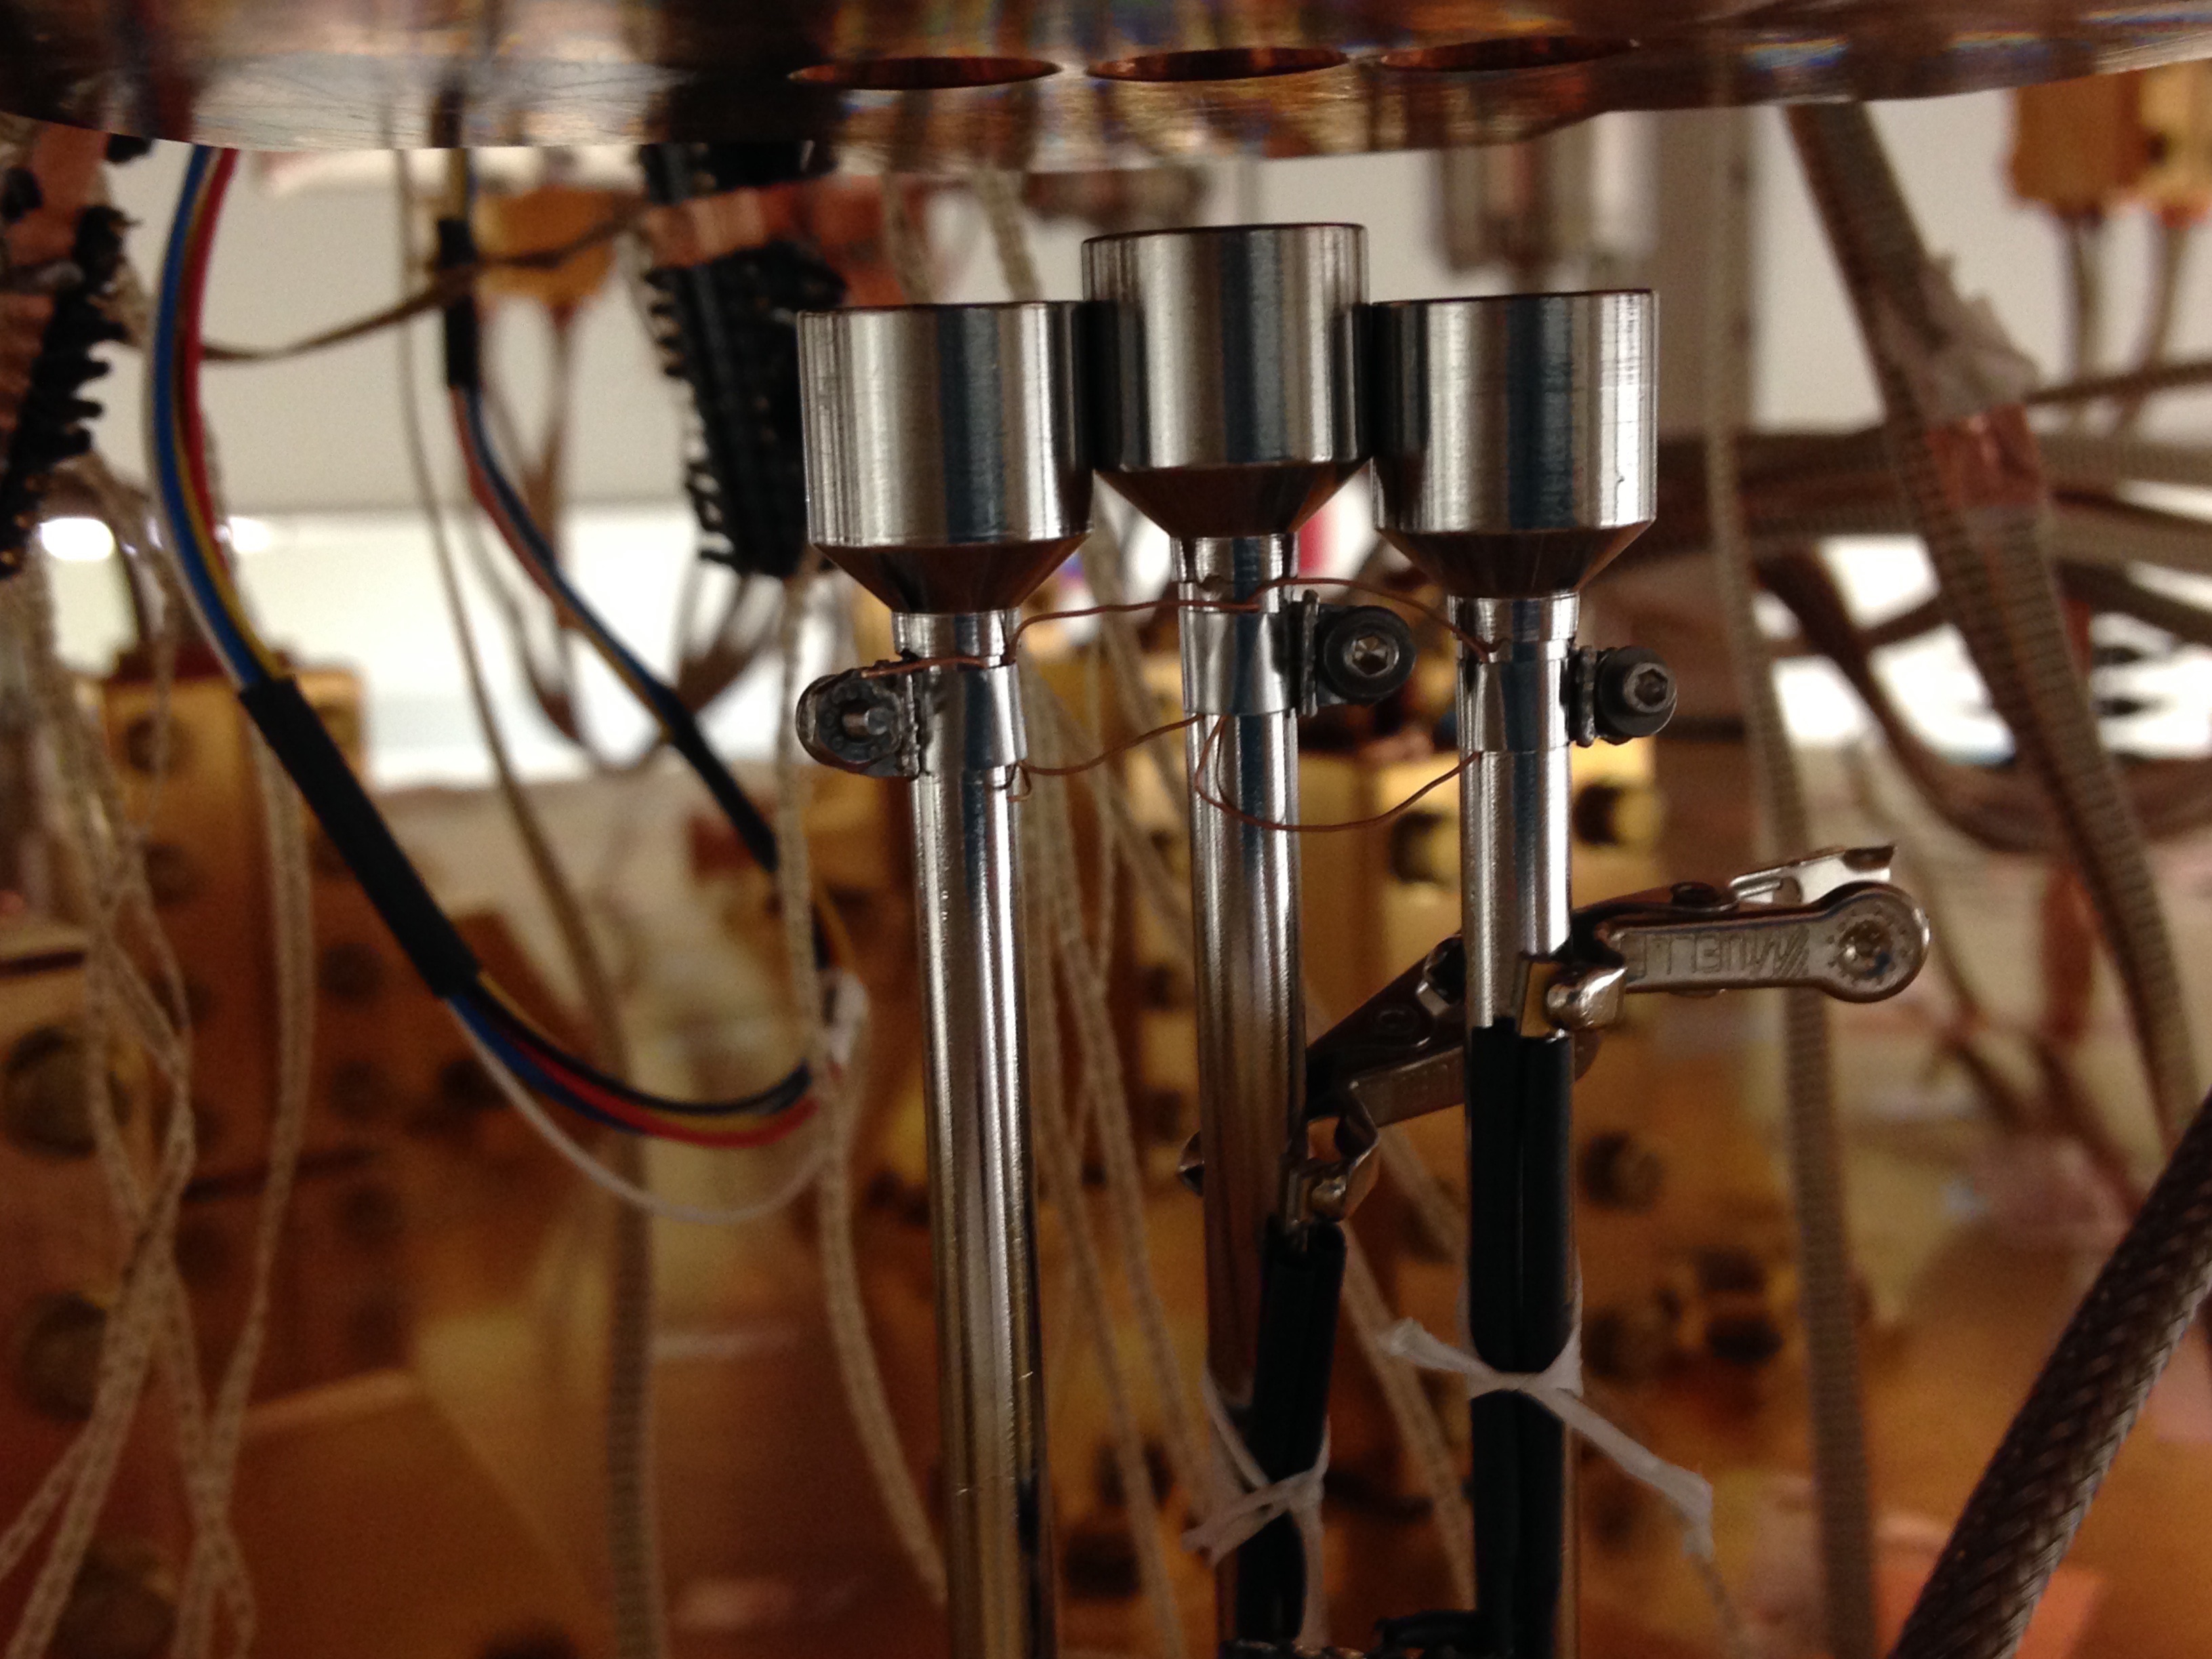
\includegraphics[width=0.8\linewidth]{Figures/ChicaneThermometers.JPG}
    \caption[The chicane thermometers.]
    {The Chicane thermometers under the 4K stage.
    These cernox thermometers are used to determine the temperature of the capsules as they leave the 4~K thermalizer into the 600~mK guide tubes.}
    \label{fig:chicane_thermometers}
\end{figure}

\subsection{Software Control of the DCS}
Diagrams to include: pictures of the thermometers, heat loads on the thermometers in different scenarios, 600 mK chicane, 4K thermalizers
\subsection{Impact on Cryostat}

Describe how the calibration affects the state of the cryostat. What are the temperature effects on the plates during the deployment.


\section{Calibration Simulation}
Describe how the simulations for the calibration system are performed. How to determine the best calibration time and effects of pileup.

Figures to include; Geant4 visualization of the sources, rates on the detectors in a calibration, rate dependence on pileup 

\section{Calibration Performance}

Describe how well the calibration system has performed? Also show different strategies for deploying the DCS.

\subsection{Calibration Strategies}

When deploying strings, it would be considerably simpler if one could deploy all the strings simultaneously down into the cryostat; however, there are multiple considerations that need to be taken into account during the operation.
Firstly, one of the main constraints is that no strings can pass through a 4-K thermalizer while it is squeezing on another string.
As the time it takes to squeeze on each set of capsules takes 10-20 minutes, this process takes hours, during which no other string can be moved through the thermalizer.
Secondly, the heat load from the calibration sources themselves is important.